\documentclass[a4paper,10pt]{article}
\usepackage{My_math_package}



\title{MATH808F - Modular Forms}
\author{Haoran Li}
\date{2020 Fall}

\makeindex[columns=2, title=Index, intoc] % Create the index

\begin{document}\sloppy % reduce overlong words

% Maketitle
\begin{titlepage}
\begin{center}
\vspace*{1cm}
\LARGE
\textbf{MATH808F - Modular Forms} \\
\vspace{2cm}
\begin{center}
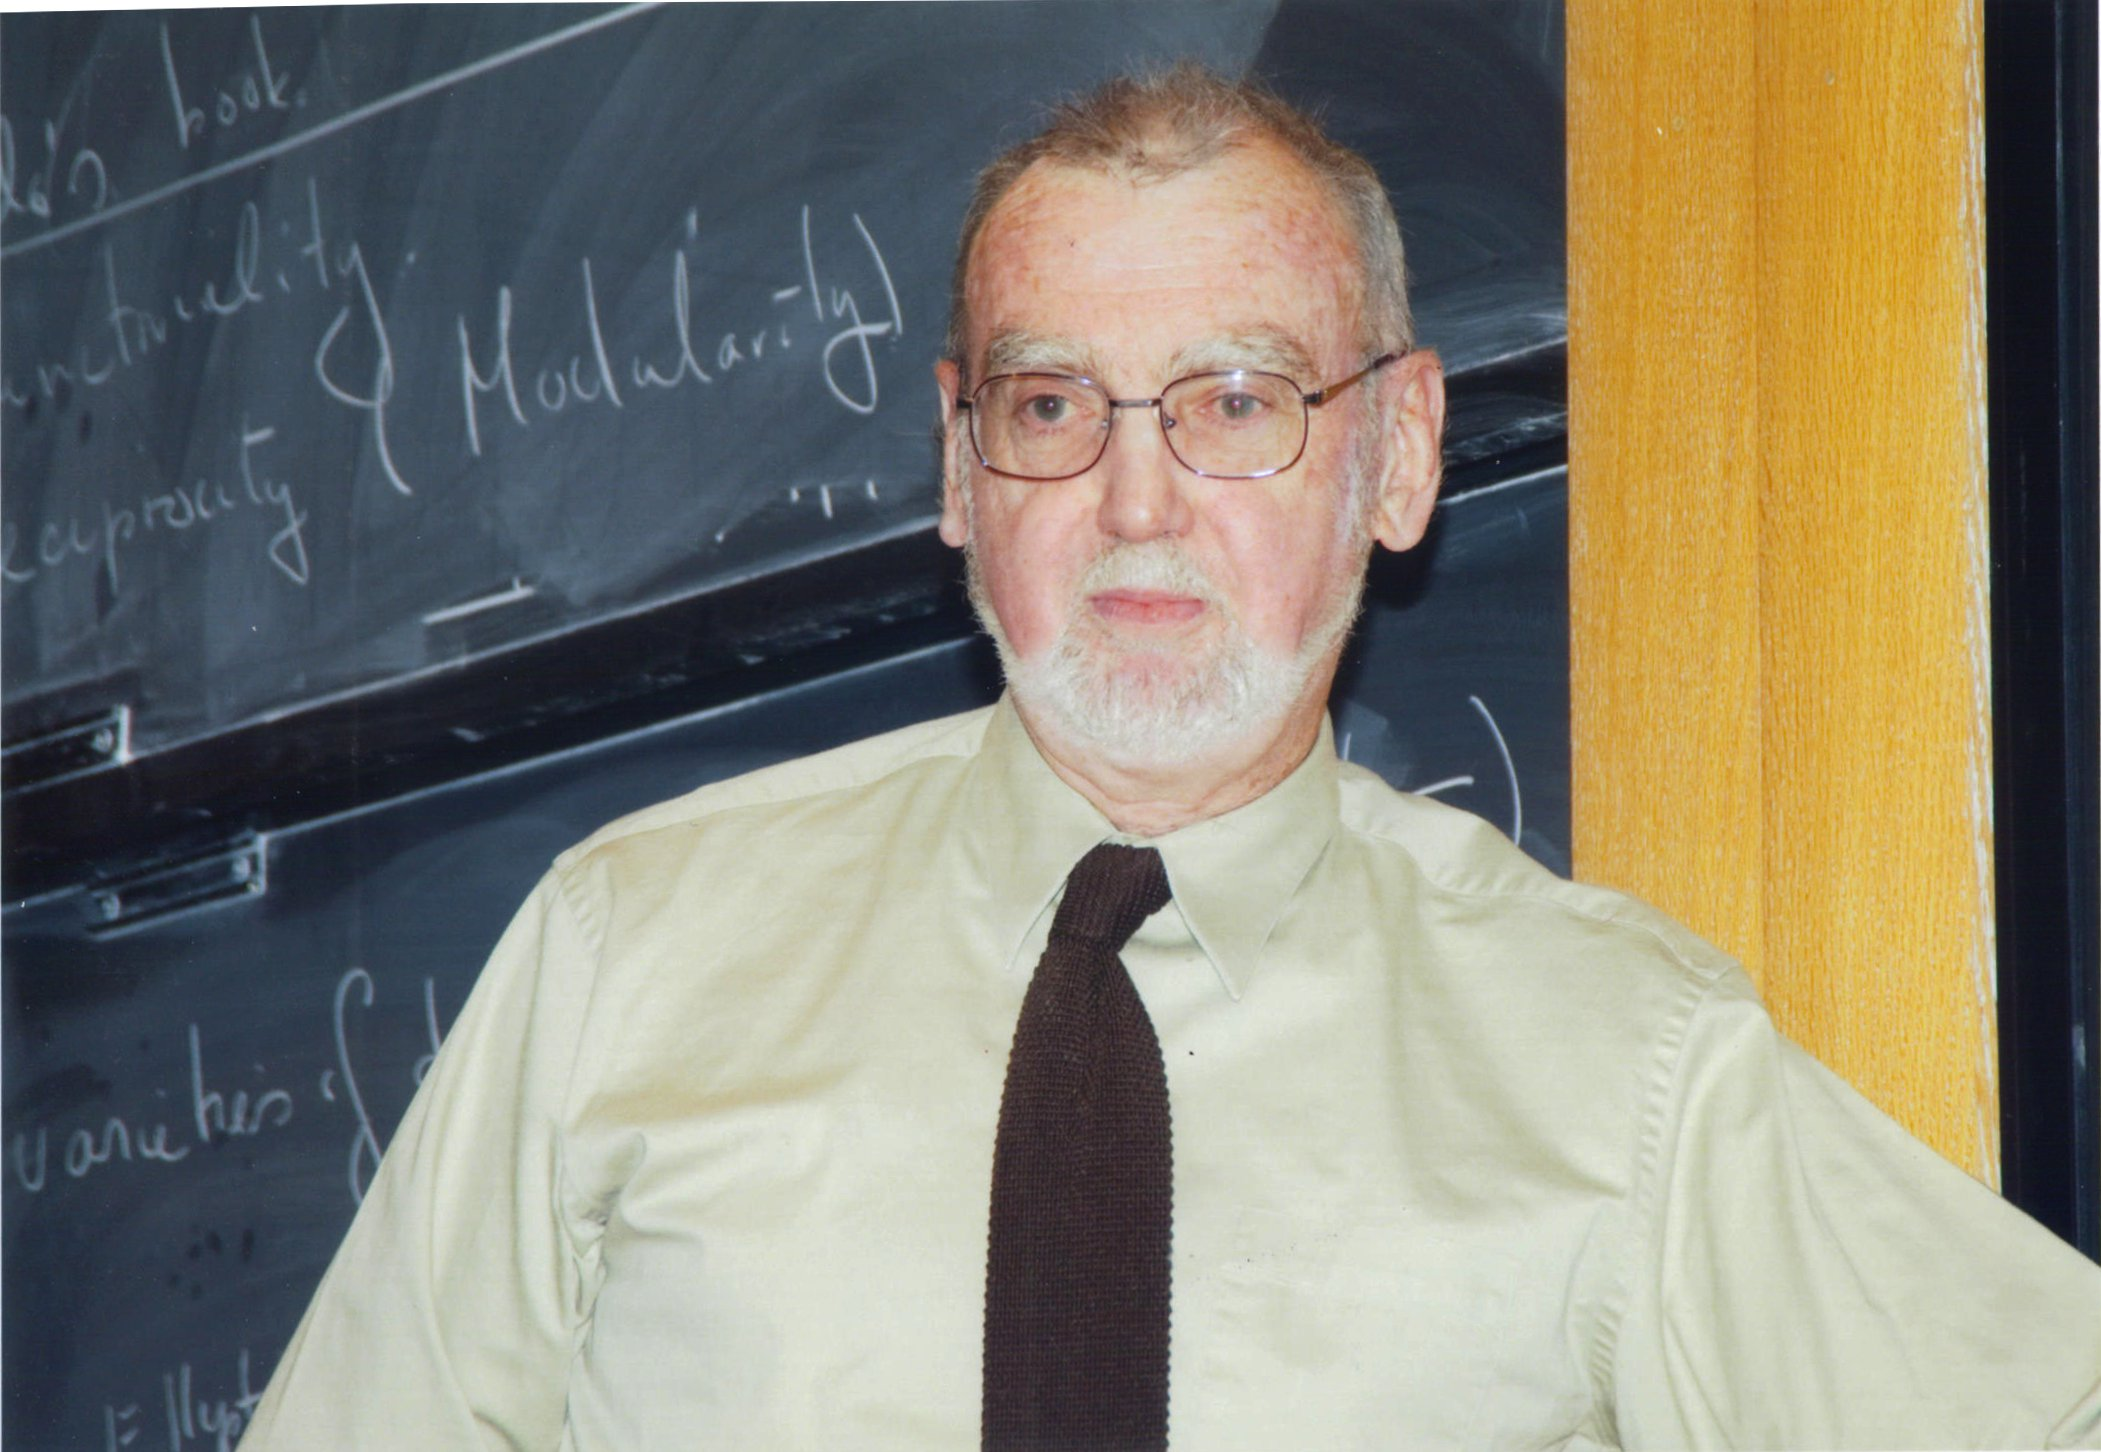
\includegraphics[width=0.5\textwidth]{Pictures/Langlands.jpg}
\end{center}
\vspace{2cm}
\normalsize
Taught by \texttt{Jingren Chi} \\
Notes taken by \texttt{Haoran Li} \\
2020 Fall \\
\vspace{2cm}
Department of Mathematics\\
University of Maryland\\
\end{center}
\end{titlepage}

\tableofcontents
\newpage

\section{Overview}
\subfile{Overview.tex}
\newpage

\section{Upper half plane}
\subfile{Upper_half_plane.tex}
\newpage

\section{Actions of Lie groups and discrete subgroups}
\subfile{Actions_of_Lie_groups_and_discrete_subgroups.tex}
\newpage

\section{Quotients of upper half plane}
\subfile{Quotients_of_upper_half_plane.tex}
\newpage

\section{Holomorphic modular forms}
\subfile{Holomorphic_modular_forms.tex}
\newpage

\section{Automorphic forms on $\GL(2,\mathbb R)$}
\subfile{Automorphic_forms_on_GL(2,R).tex}
\newpage

\section{Growth conditions and fundamental estimates}
\subfile{Growth_conditions_and_fundamental_estimates.tex}
\newpage

\section{Cuspidal spectrum}
\subfile{Cuspidal_spectrum.tex}
\newpage

\section{Representations of $\GL(2,\mathbb R)$}
\subfile{Representations_of_GL(2,R).tex}
\newpage

\section{Hecke operators}
\subfile{Hecke_operators.tex}
\newpage

\section{Hecke algebras for congruence subgroups}
\subfile{Hecke_algebras_for_congruence_subgroups.tex}
\newpage

\section{Automorphic forms on $GL_2(\mathbb A)$}
\subfile{Automorphic_forms_on_GL2(A).tex}
\newpage

\section{Automorphic representations on $GL_2(\mathbb A)$}
\subfile{Automorphic_representations_on_GL2(A).tex}
\newpage

\section{Representations of $\GL_2$ over $p$-adic fields}
\subfile{Representations_of_GL2_over_p-adic_fields.tex}
\newpage

\section{Global Whittaker model and multiplicity one}
\subfile{Global Whittaker model and multiplicity one.tex}
\newpage

\section{L-functions of modular forms}
\subfile{L-functions_of_modular_forms.tex}
\newpage

\section{Abelian L-functions}
\subfile{Abelian L-functions.tex}
\newpage

\section{Automorphic L-functions of $\GL_2$}
\subfile{Automorphic L-functions of GL_2.tex}
\newpage

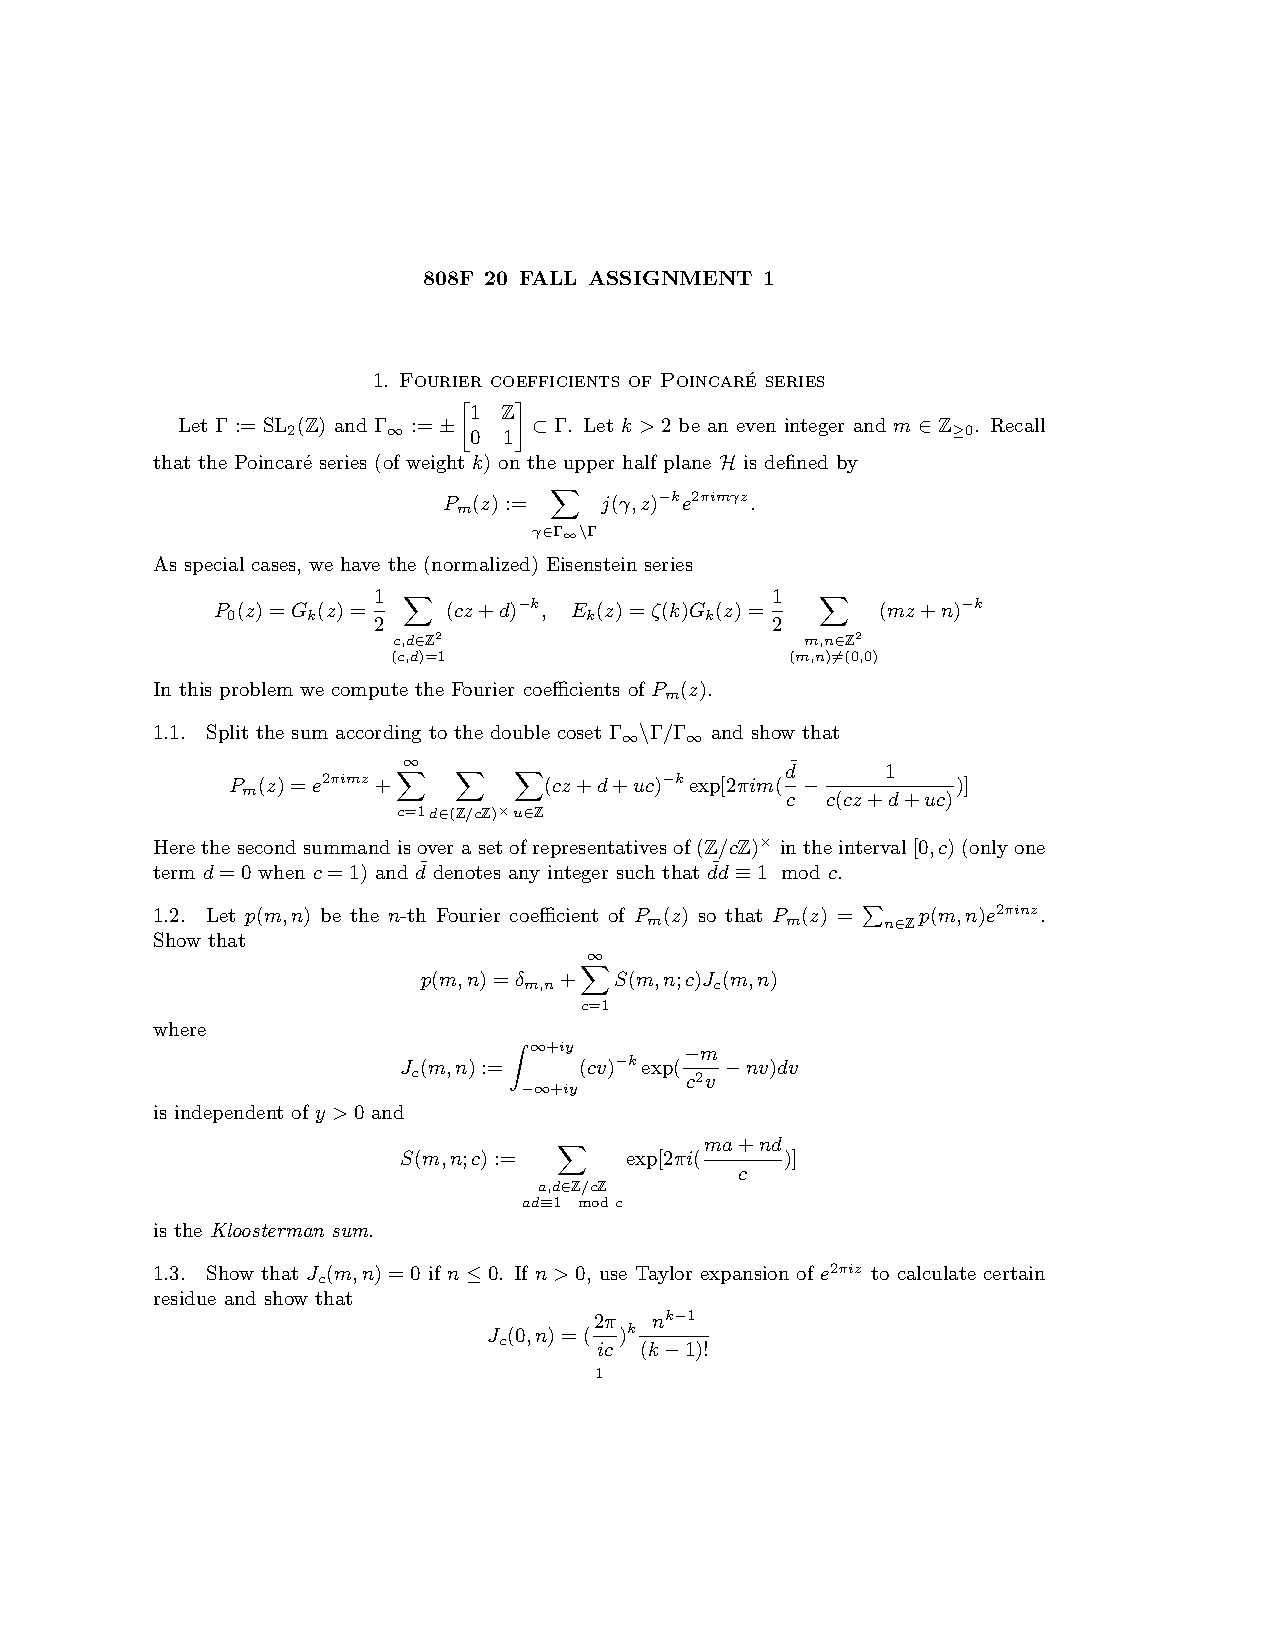
\includepdf[pages=-]{HW1.pdf}
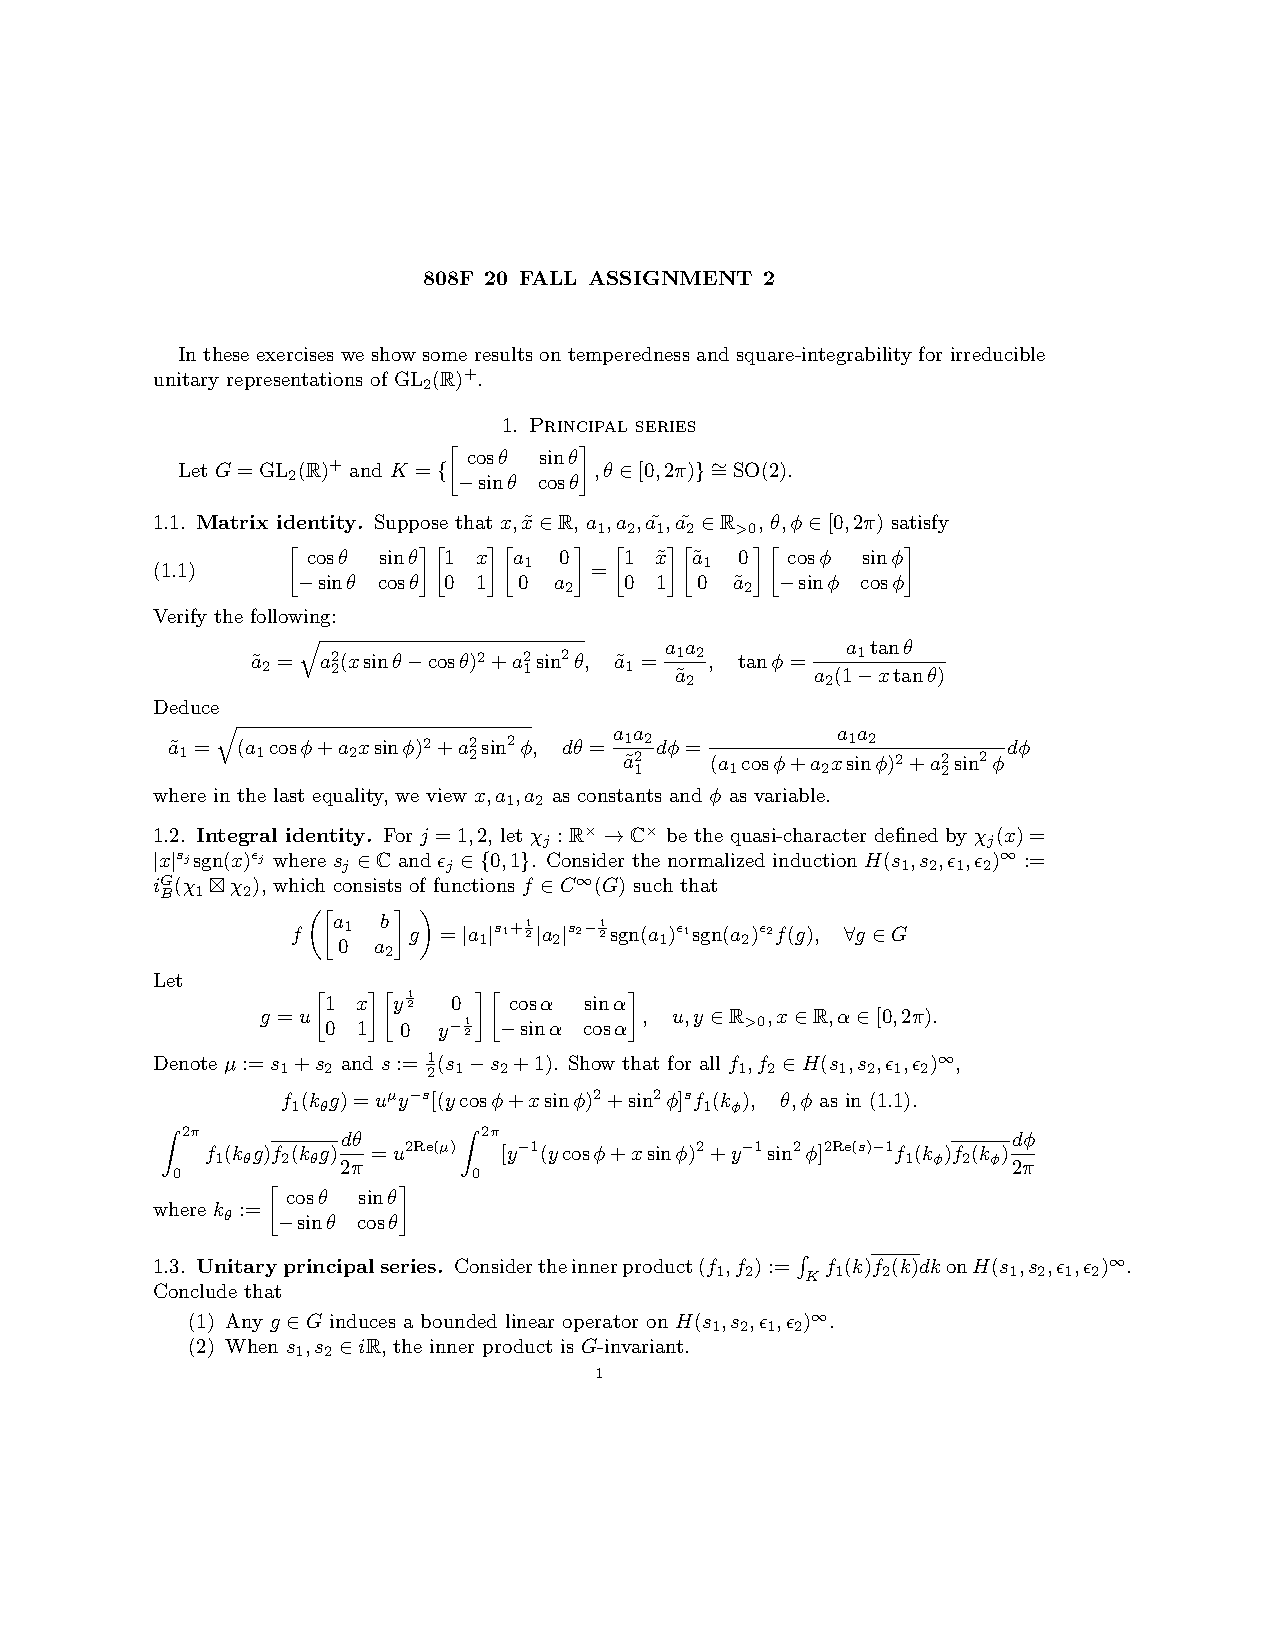
\includepdf[pages=-]{HW2.pdf}

\begin{thebibliography}{}

\bibitem{A First Course in Modular Forms} 
\textit{A First Course in Modular Forms} - Fred Diamond, Jerry Shurman

\end{thebibliography}

\printindex
\newpage

\end{document}